\documentclass[bluish,slideColor,colorBG,pdf]{prosper}
\hypersetup{pdfpagemode=FullScreen}
\usepackage{graphicx}
\usepackage{multirow}
\def\baselinestretch{1.0}
\setlength{\topmargin}{-60pt}
\setlength{\textheight}{460pt}
\setlength{\oddsidemargin}{0pt}
\setlength{\evensidemargin}{0pt}
\setlength{\textwidth}{660pt}
\setlength{\footskip}{0pt}
\parindent 0.3in
\hyphenpenalty=10000
\tolerance=10000
\pagestyle{empty}

\def\Prob{{\rm Prob\;}}
\def\prob{{\rm \;Prob\;}}

\title{Week 3:  Parsimony variants, compatibility, statistics and parsimony}
\author{Genome 570}
\institution{January, 2016}

\begin{document}

\maketitle

\begin{slide}[Replace]{Weighting using a function}

Suppose that each step is to be weighted $1/(n+2)$ if the character
has a total of $n$ steps.
\bigskip

Then the total weight of steps when there are $n$ steps in that character is
$n \times 1/(n+2)$ which is  $n/(n+2)$
\bigskip

\begin{center}
\begin{tabular}{c | l l}
\multicolumn{1}{c}{Total steps in} & \multicolumn{1}{c}{Weight of} &
\multicolumn{1}{c}{Total weight} \\
\multicolumn{1}{c}{the character} & \multicolumn{1}{c}{each step} &
\multicolumn{1}{c}{of all steps} \\
\hline
0 & 0.5\raisebox{2pt}{\strut}  & 0 \\
1 & 0.3333 & 0.3333\\
2 & 0.25  & 0.5 \\
3 & 0.2 & 0.6 \\
4 & 0.1667 & 0.6667 \\
5 & 0.142857 & 0.71428
\end{tabular}
\end{center}

The rationale for doing this is to somewhat discount the information from
more rapidly changing characters.

\end{slide}

\begin{slide}[Replace]{Successive weighting}
\bigskip

J.S. Farris suggested (1969):

\begin{enumerate}
\item Infer a tree with unweighted parsimony
\item Calculate weights for each character (or site) based on the
number of changes in that character on that tree
\item Use those weights to infer a new tree
\item Unless the tree hasn't changed, go back to step 2.
\end{enumerate}
\bigskip

This method, which was put forward in the first modern quantitative paper
on weighting, was intended to discount rapidly-evolving characters.

\end{slide}

\begin{slide}[Replace]{Successive weighting}

\noindent
There are 15 possible unrooted trees, which fall into
5 types according to how many changes they have in each character.
The table shows the total weighted number of changes when each
tree type is evaluated using the weights implied by the 5 different
tree types.
\bigskip

{\parindent=-0.1in
\renewcommand{\arraystretch}{1.3}
\begin{tabular}{| c | c | c | c c c c c |} 
\hline
number & have pattern & type & \multicolumn{5}{c |}{tree type used for weights}\\
of trees & of changes: & of tree & I & II & III & IV & V \\ 
\hline
1 & (1,1,1,2,2,1) & I & 2.333 & 2.250 & 2.167 & 2.417 & 2.083\\
2 & (1,2,1,2,2,1) & II & 2.667 & 2.500 & 2.500 & 2.667 & 2.333\\
2 & (2,1,2,2,2,1) & III & 3.000 & 2.917 & 2.667 & 2.917 & 2.583\\
3 & (2,2,2,1,1,1) & IV & 2.833 & 2.667 & 2.500 & 2.500 & 2.333\\
7 & (2,2,2,2,2,1) & V & 3.333 & 3.167 & 3.000 & 3.167 & 2.833\\
\hline
\end{tabular}
}

From this table you can figure out what the sequence of trees will be
if you start from one of these types.  Do you get different ultimate outcomes?

\end{slide}

\begin{slide}[Replace]{Ties in successive weighting}

\noindent
An example of successive weighting that would show
the difficulty it has in detecting ties.
The table shows the total weighted number of changes when each
tree type is evaluated using the weights implied by the different
tree types.
\bigskip

\begin{center}
\renewcommand{\arraystretch}{1.3}
\begin{tabular}{| c | c | c | c c c |}
\hline
number & have pattern & type & \multicolumn{3}{c |}{tree type used for weights}\\
of trees & of changes: & of tree & I & II & III \\
\hline
1 & (1,1,2,2) & I & 1.667 & 1.833 & 1.5 \\
1 & (2,2,1,1) & II & 1.833 & 1.667 & 1.5 \\
1 & (2,2,2,2) & III & 2.333 & 2.333 & 2 \\
\hline
\end{tabular}
\end{center}

\end{slide}

\begin{slide}[Replace]{Nonsuccessive weighting}
\bigskip

We can use a different algorithm to avoid the issue of dependence
on starting point which is seen in successive weighting:
\medskip

\begin{itemize}
\item Search over tree space in the usual way
\item For each tree, evaluate the number of steps in each character (or site)
\item Calculate the weight for the character from its number of steps on the
current tree in the search.
\item Add up the weighted steps across characters to evaluate that tree.
\end{itemize}
\bigskip

This is equivalent to looking only at the diagonals in the preceding tables
of trees.  Weights are never based on a different tree.

\end{slide}

\begin{slide}[Replace]{Evaluating compatibility with 0/1 characters}

E. O. Wilson ({\it Systematic Zoology, 1965}) pointed out that
for two characters,
if all four combinations  $00$, $01$, $10$ and $11$ exist in one or
another species, the two characters must be incompatible with each
other, in the sense that there can be no tree on which they each change
only once (so the derived state is uniquely derived).
\medskip

\begin{center}
\parbox[t]{1.0in}{
Compatible characters\\

\begin{tabular}{c | c c |}
  & 0  & 1 \\
\hline
 0  &\raisebox{2pt}{\strut} X  & X \\
 1  &    & \raisebox{2pt}{\strut}X \\
\hline
\end{tabular}
} \hspace{1.0in}
\parbox[t]{1.0in}{
Incompatible characters\\

\begin{tabular}{c | c c |}
  & 0  & 1 \\
\hline
 0  & \raisebox{2pt}{\strut}X  & X \\
 1  & \raisebox{2pt}{\strut}X  & X \\
\hline
\end{tabular}
}
\end{center}
\medskip

The logic is straightforward: to originate a new combination requires
a step in one character (or both).  With four combinations there are 3 steps
required, one more than the number that would be needed if both characters were
incompatible.  (In genomics this is called the ``three-gamete condition'' --
out of the four possibilities there must be three or fewer for there to have
been no recombination and no recurrent mutations).

\end{slide}

\begin{slide}[Replace]{Data example for compatibility}

\noindent
The data set Table 1.1 with an added species all of
whose characters are 0.
\bigskip

\begin{center}
\renewcommand{\arraystretch}{1.3}
\begin{tabular}{l | l | c c c c c c |}
\cline{3-8}
\multicolumn{2}{c}{}& \multicolumn{6}{|c|}{Characters}\\
\multicolumn{2}{r |}{Species} & 1 & 2 & 3 & 4 & 5 & 6 \\
\cline{2-8}
&Alpha & 1 & 0 & 0 & 1 & 1 & 0\\
&Beta  & 0 & 0 & 1 & 0 & 0 & 0\\
&Gamma & 1 & 1 & 0 & 0 & 0 & 0\\
&Delta & 1 & 1 & 0 & 1 & 1 & 1\\
&Epsilon & 0 & 0 & 1 & 1 & 1 & 0\\
&Omega & 0 & 0 & 0 & 0 & 0 & 0 \\
\cline{2-8}
\end{tabular}
\end{center}

\end{slide}

\begin{slide}[Replace]{The compatibility matrix for this data set}

\centerline{\includegraphics[width=2.4in]{fig8-1.ydraw}}
\bigskip

The darkly-shaded boxes are the combinations that are compatible.

\end{slide}

\begin{slide}[Replace]{The Pairwise Compatibility Theorem}
{~~}

\vfill

\centerline{
\fbox{\parbox{3.0in}{A set $S$ of characters has all
pairs of characters compatible with each other if and only if all of the
characters in the set are jointly compatible (in that there
exists a tree with which all of them are compatible).}}
}
\bigskip

This theorem is true, given the right conditions, which we will explain.

\vfill

\vfill

\end{slide}

\begin{slide}[Replace]{The compatibility graph}

\centerline{Maximal cliques?  Largest?}
{~~}
\bigskip

\centerline{\includegraphics[width=2.4in]{fig8-2.ydraw}}

\end{slide}

\begin{slide}[Replace]{One of the cliques it contains}

{~~}
\vspace{0.24in}
\bigskip

\centerline{\includegraphics[width=2.4in]{fig8-2a.ydraw}}

\end{slide}

\begin{slide}[Replace]{A maximal clique}

{~~}
\vspace{0.24in}
\bigskip

\centerline{\includegraphics[width=2.4in]{fig8-2b.ydraw}}

\end{slide}

\begin{slide}[Replace]{The largest maximal clique}

{~~}
\vspace{0.24in}
\bigskip

\centerline{\includegraphics[width=2.4in]{fig8-2c.ydraw}}

\end{slide}

\begin{slide}[Replace]{Making the tree by ``tree popping'' }
(for clique $\mathsf\{1, 2, 3, 6\}$)

\centerline{\includegraphics[width=4.0in]{fig8-3a.ydraw}}

\end{slide}

\begin{slide}[Replace]{Making the tree by ``tree popping'' }
(for clique $\mathsf\{1, 2, 3, 6\}$)

\centerline{\includegraphics[width=4.0in]{fig8-3b.ydraw}}

\end{slide}

\begin{slide}[Replace]{Making the tree by ``tree popping'' }
(for clique $\mathsf\{1, 2, 3, 6\}$)

\centerline{\includegraphics[width=4.0in]{fig8-3c.ydraw}}

\end{slide}

\begin{slide}[Replace]{Making the tree by ``tree popping'' }
(for clique $\mathsf\{1, 2, 3, 6\}$)

\centerline{\includegraphics[width=4.0in]{fig8-3d.ydraw}}

\end{slide}

\begin{slide}[Replace]{Unknown states and compatibility}
\bigskip

\noindent
A data set that has all pairs of characters compatible, but which
cannot have all characters compatible with the same tree.  This violates
the Pairwise Compatibility Theorem, owing to the unknown ("?") states.
\bigskip

\begin{center}
\renewcommand{\arraystretch}{1.3}
\begin{tabular}{l | c c c |}
\cline{2-4}
Alpha & 0 & 0 & 0 \\
Beta & ? & 0 & 1 \\
Gamma & 1 & ? & 0 \\
Delta & 0 & 1 & ? \\
Epsilon & 1 & 1 & 1 \\
\cline{2-4}
\end{tabular}
\end{center}

\end{slide}

\begin{slide}[Replace]{Multiple character states and compatibility}

\bigskip

\noindent
Walter Fitch's set of nucleotide sequences that have each pair of
sites compatible, but which are not all compatible with the same tree.
\bigskip


\begin{center}
\renewcommand{\arraystretch}{1.3}
\begin{tabular}{l | c c c |}
\cline{2-4}
Alpha & A & A & A \\
Beta & A & C & C \\
Gamma & C & G & C \\
Delta & C & C & G \\
Epsilon & G & A & G \\
\cline{2-4}
\end{tabular}
\end{center}

\end{slide}

\begin{slide}[Replace]{Haplotypes of SNPs in a simulated population}

\centerline{\includegraphics[height=3in]{Dhaplotypes.idraw}}

\end{slide}

\begin{slide}[Replace]{Values of the LD measure $\mathsf{|D'|}$ }

\centerline{\includegraphics[height=3in]{GOLD2.idraw}}

\end{slide}

\begin{slide}[Replace]{Two of the pairs of SNPs that show $\mathsf{|D'| = 1}$ }

\centerline{\includegraphics[height=3in]{Dhaplotypes2.idraw}}

\end{slide}

\begin{slide}[Replace]{Transition probabilities in a two-state model}

{\ptsize{8}
In a symmetric two-state model with rate of change $\mathsf{r}$ per unit time,
where\\
\begin{tabular}{c c l}
\parbox[b]{0.8in}{\includegraphics[width=0.5in]{01.ydraw}} &  \hspace{0.1in}  we have \hspace{0.1in}
&\ptsize{12}{
$\prob\mathsf{(1\;|\;0, t, r)\  = \ \frac{1}{2}\left(1 - e^{-2\,r\,t} \right)}
$}
\end{tabular}
}

\centerline{\includegraphics[width=2.0in]{twostate.ydraw}}
\medskip

When $\ \mathsf{r\,t}\ $ is small then to very good approximation the probability
of the events in the branch is $\ \mathsf{r\,t}\ $ or $\ \mathsf{1\;-\;r\,t}\ $.
The latter is nearly $\ \mathsf{1}$.

\end{slide}

\begin{slide}[Replace]{Likelihood and parsimony}

Approximating all the terms $\mathsf{~1 - r\,t_i~}$ by $\mathsf{~1~}$, we
find the probabilities of these data for the four possible choices of interior node states:

\begin{tabular}{c c}
$\begin{array}{c c}
\multirow{15}{*}{\includegraphics[width=1.5in]{trees01.idraw}} & \\
& \\
& \mathsf{\frac{1}{2} (r\,t_3) (r\,t_4)} \\
& \\
& \\
& \\
 & \mathsf{\frac{1}{2} (r\,t_5) } \\
& \\
& \\
& \\
 & \mathsf{\frac{1}{2} (r\,t_1) (r\,t_2) (r\,t_5) (r\,t_3) (r\,t_4)} \\
& \\
& \\
& \\
 & \mathsf{\frac{1}{2} (r\,t_1) (r\,t_2)}
\end{array}
$
& {~~~~~}
\end{tabular}

\end{slide}

\begin{slide}[Replace]{Likelihood and parsimony}

\noindent
\hspace*{0.0in}\hspace{-0.3in}\[
\begin{array}{c c  l}
\mathsf{L} & \mathsf{=}  & \prob(\mbox{Data}|\mbox{Tree})\\
  & & \\
  & = & \prod\limits_{\mathsf{i=1}}^{\mbox{$\rm chars$}}
               \sum\limits_{\begin{array}{l}\mbox{$\rm recon-$}\\
                                            \mbox{$\rm structions$}\end{array}}              \left(\mathsf{\frac{1}{2} \prod\limits_{j=1}^B
        \left\{
            \begin{array}{c l}
            r_i t_j &  \mbox{if~this~character~changes}\\
            1 - r_i t_j &  \mbox{if~it~does~not~change}
            \end{array}
         \right\} }\right)
\end{array}
\]
\bigskip

The sum is over all reconstructions of changes in that character that
result in the observed states at the tips of the tree.  It is {\it not} just
over all most parsimonious reconstructions of changes.
\bigskip

We will see (later in the course) that maximizing the likelihood is a Good
Thing.  We want to show that in the case where changes are infrequent,
there is a relationship between that and minimizing the (weighted) parsimony
score, and what the proper weights turn out to be.


\end{slide}

\begin{slide}[Replace]{approximating ... }

\noindent
If we toss out, in each character, all the terms that have more than the
smallest possible number of terms $~\mathsf{r t}$,
for each character ($\mathsf{i}$) the likelihood is approximately the
product over all branches (the $\mathsf{j}$th of which has length $\
\mathsf{t_j}$)
\[
\mathsf{\frac{1}{2}\,\prod_{i=1}^B \left(r_i t_j\right)^{n_{ij}}.}
\]

\noindent
where $\mathsf{~n_{ij}~}$ is either $\mathsf{~0~}$ or $\mathsf{~1~}$,
for all characters the likelihood is then approximately
\[
\mathsf{L\ \ \simeq\ \ \prod_{i=1}^{\mbox{{$\rm chars$}}}\left( \frac{1}{2}\, \prod_{j=1}^{\mbox{$\rm branches$}} \left(r_it_j\right)^{n_{ij}}\;\right)}.
\]

\noindent
Tossing out the $~\mathsf{1/2}~$ terms and taking logarithms, if the number of
changes in character $\ \mathsf{i}\ $ in branch $\ \mathsf{j}\ $ is $\
\mathsf{n_{ij}}$,
\[
\mathsf{- \ln L\ \ \simeq\ \ \sum_{i=1}^{\mbox{$\rm chars$}}\; \sum_{j=1}^{\mbox{$\rm branches$}} n_{ij}\left( - \ln \left(r_it_j\right)\right).}
\]

\end{slide}

\begin{slide}[Replace]{Weights and likelihood}

Probabilities of change and resulting weights for an imaginary case.

\begin{center}
\begin{tabular}{c l r r}
Character & $\mathsf{r_i\,t_j}$ & changes & total weight\\
   &   &   & \\
1 & 0.01 & 1 &  4.605  \\
2 & 0.01 & 2 &  9.210  \\
3 & 0.00001 & 1 & 11.519
\end{tabular}
\end{center}

\end{slide}

\begin{slide}[Replace]{with one-tenth as much change ... }

\begin{center}  
\begin{tabular}{c l r r}
Character & $\mathsf{r_i\,t_j}$ & changes & total weight\\
   &   &   & \\
1 & 0.001 & 1 &  6.908  \\
2 & 0.001 & 2 &  13.816\\
3 & 0.000001 & 1 & 13.816
\end{tabular}
\end{center} 

\end{slide}

\begin{slide}[Replace]{ ... and with one-tenth less again}

\begin{center}
\begin{tabular}{c l r r}
Character & $\mathsf{r_i\,t_j}$ & changes & total weight\\
   &   &   & \\
1 & 0.0001 & 1 &  9.210  \\
2 & 0.0001 & 2 & 18.421  \\
3 & 0.0000001 & 1 & 16.118
\end{tabular}
\end{center}

\end{slide}

\begin{slide}[Replace]{Trees, steps, and patterns}

\centerline{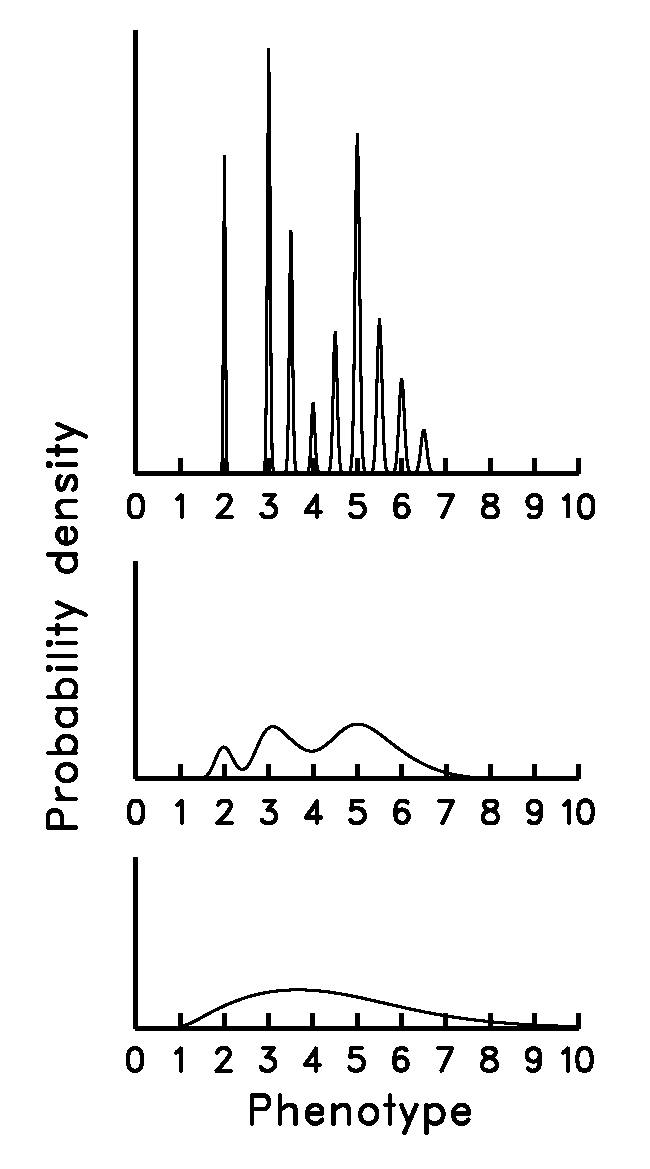
\includegraphics[width=2.2in]{fig9-2.ydraw}}
\medskip

This table shows how many changes of state (steps) are needed for each
of the 16 possible character patterns on each of the three unrooted tree
topologies, under a parsimony criterion.

\end{slide}

\begin{slide}[Replace]{Trees, steps, and patterns with DNA}

\centerline{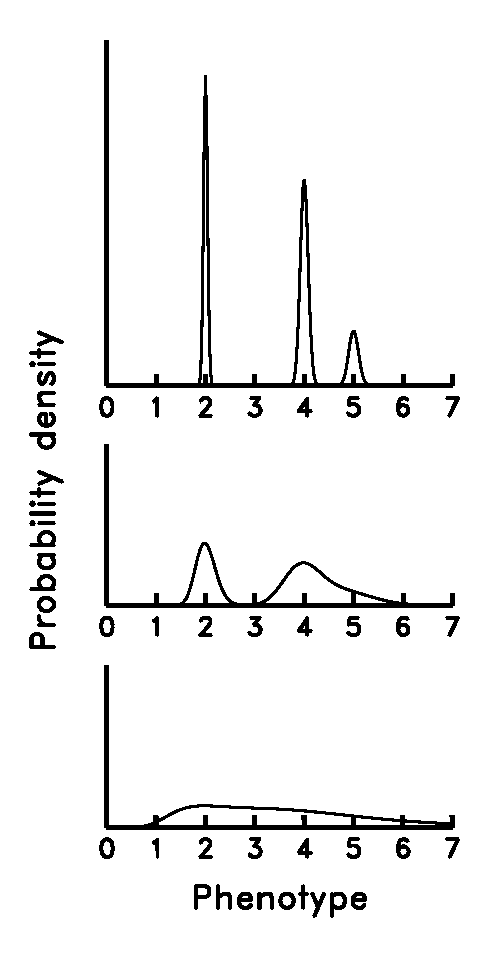
\includegraphics[width=2.0in]{fig9-1.ydraw}}

\end{slide}

\begin{slide}[Replace]{Parsimony and patterns}
\bigskip

Ignoring all the patterns that have the same number of steps on all topologies,
the ones that matter to a parsimony method have one of these three sums:

\[
\mathsf{n_{xxyy} + 2n_{xyxy} + 2n_{xyyx}\  = \ 2(n_{xxyy}+n_{xyxy}+n_{xyyx}) - n_{xxyy}}
\]
\medskip

\[
\mathsf{2n_{xxyy} + n_{xyxy} + 2n_{xyyx} \ = \ 2(n_{xxyy}+n_{xyxy}+n_{xyyx}) - n_{xyxy}}
\medskip
\]

\[
\mathsf{2n_{xxyy} + 2n_{xyxy} + n_{xyyx} \ = \ 2(n_{xxyy}+n_{xyxy}+n_{xyyx}) - n_{xyyx}.}
\]

\end{slide}

\end{document}
